\documentclass[conference]{IEEEtran}
\IEEEoverridecommandlockouts

\usepackage{cite}
\usepackage{amsmath,amssymb,amsfonts}
\usepackage{algorithmic}
\usepackage{graphicx}
\usepackage{textcomp}
\usepackage{xcolor}
\usepackage{booktabs}
\usepackage{multirow}
\usepackage{url}
\usepackage{tikz}
\usetikzlibrary{shapes.geometric, arrows.meta, positioning, calc, fit, backgrounds}

\begin{document}

\title{Skill Gap Analysis and Personalized Career Development Using Gradient Boosted Decision Trees}

\author{
    \IEEEauthorblockN{
        Yenura S. Karunanayaka\IEEEauthorrefmark{1},
        D. T. D. Perera\IEEEauthorrefmark{2},
        Dulnith K. D.\IEEEauthorrefmark{3}, and
        K. G. Savinda N. Perera\IEEEauthorrefmark{4}
    }
    \IEEEauthorblockA{
        Faculty of Computing, Sri Lanka Institute of Information Technology (SLIIT), Malabe, Sri Lanka\\
        Email: \IEEEauthorrefmark{1}it22306272@my.sliit.lk (ID: IT22306272),
               \IEEEauthorrefmark{2}it22089236@my.sliit.lk (ID: IT22089236),\\
               \IEEEauthorrefmark{3}it22094872@my.sliit.lk (ID: IT22094872),
               \IEEEauthorrefmark{4}it22027610@my.sliit.lk (ID: IT22027610)
    }
}

\maketitle

\begin{abstract}
Traditional candidate rejection in enterprise recruitment functions as an uninformative dead end, discarding unselected applicants without diagnostic feedback or structured upskilling guidance. In this paper, we present the architecture, algorithmic design, and empirical validation of Component 4 of the RecruitAI ecosystem: an intelligent skill gap analysis and personalized career development microservice operating on Port 8004. The engine ingests candidate qualification vectors and evaluates them against target IT job roles via a two-stage fuzzy string and semantic matching algorithm, strictly distinguishing required from optional competencies and computing a normalized gap severity index $G_s$. To model candidate suitability under hiring policy benchmarks, we train a Gradient Boosted Decision Tree (GBDT) classifier across 20,000 candidate records characterized by 67 engineered features spanning skill coverage ratios, experience tenure, education tiers, and role encodings. Crucially, because longitudinal corporate hiring telemetry was unavailable, the model is scientifically evaluated on a rule-based hireability target rather than real-world employment decisions. Our GBDT ensemble achieves an accuracy of 91.50\%, an $F_1$-score of 0.8670, and an area under the ROC curve ($\text{ROC-AUC}$) of 0.9763, substantially outperforming Random Forest and Logistic Regression baselines. The system maps identified skill deficiencies to a curated 47-course catalog, synthesizes a monthly learning roadmap paced realistically at 2 skills per month, and navigates a Directed Acyclic Graph (DAG) of vertical and lateral career transitions.
\end{abstract}

\begin{IEEEkeywords}
Skill Gap Analysis, Career Development, Gradient Boosted Decision Trees, Learning Pathway Recommendation, Career Mobility DAG, Recommender Systems, Educational Data Mining.
\end{IEEEkeywords}

\section{Introduction}
In competitive technical recruitment, over 95\% of applicants for any given software engineering or data architecture role are ultimately unselected~\cite{sackett2022revisiting}. In standard corporate workflows, rejected candidates receive generic, uninformative rejection templates. This practice squanders valuable candidate engagement, provides zero guidance on addressable skill deficiencies, and forces job seekers into repetitive, unfocused trial-and-error applications~\cite{zhang2023job}. Concurrently, enterprise talent acquisition teams struggle to cultivate long-term talent pools, repeatedly re-advertising vacancies rather than nurturing high-potential applicants who narrowly missed specific technical thresholds.

At the same time, automated career guidance tools frequently suffer from simplistic matching heuristics. Most existing platforms merely compute lexical differences between resumes and job postings, failing to prioritize mandatory core requirements over secondary preferred skills. Furthermore, when generating learning recommendations, automated tools routinely produce overwhelming, unprioritized lists of online courses that disregard human cognitive limits and realistic professional learning timelines~\cite{ricci2015recommender}.

To solve these systemic shortcomings, this paper presents Component 4 of the RecruitAI ecosystem: a machine learning-driven skill gap diagnostic and personalized career navigation engine. The primary contributions of this paper are:
\begin{enumerate}
    \item \textbf{Two-Stage Fuzzy Gap Diagnosis}: We implement a fuzzy string and semantic matching pipeline that isolates missing technical skills while strictly differentiating non-negotiable core requirements from optional competencies.
    \item \textbf{Normalized Gap Severity Index ($G_s$)}: We formulate a mathematically bounded metric quantifying candidate distance from target job expectations.
    \item \textbf{67-Feature GBDT Hireability Modeling}: We engineer a comprehensive 67-dimensional feature space and train a Gradient Boosted Decision Tree ensemble achieving $\text{ROC-AUC} = 0.9763$ on a 20,000-record benchmark, providing clear scientific clarity regarding rule-based policy targets.
    \item \textbf{Realistic Monthly Learning Pathways}: We map identified skill gaps to an indexed 47-course catalog, generating structured monthly upskilling timelines paced at 2 skills per month ($T = \lceil |\mathcal{G}| / 2 \rceil$).
    \item \textbf{Directed Acyclic Graph (DAG) Career Lattice}: We formulate a multi-tier career transition graph supporting vertical promotional ladders and lateral cross-skilling transitions across 20 canonical IT roles.
\end{enumerate}

\begin{figure*}[t]
\centering
\begin{tikzpicture}[
    node distance=0.8cm and 1.2cm,
    box/.style={rectangle, draw=blue!80!black, fill=blue!5, thick, rounded corners=3pt, align=center, inner sep=6pt, font=\footnotesize},
    mod/.style={rectangle, draw=purple!80!black, fill=purple!10, thick, rounded corners=4pt, align=center, inner sep=6pt, font=\footnotesize\bfseries},
    eval/.style={rectangle, draw=orange!80!black, fill=orange!10, thick, rounded corners=3pt, align=center, inner sep=6pt, font=\footnotesize},
    out/.style={rectangle, draw=green!70!black, fill=green!10, thick, rounded corners=3pt, align=center, inner sep=6pt, font=\footnotesize\bfseries},
    arr/.style={-{Stealth[scale=0.9]}, thick, color=black!80}
]

% Inputs
\node[box] (input) {\textbf{Candidate Evaluation Profile}\\Verified Skills $\mathcal{S}_{cand}$, Experience $E$,\\Education $D, F$ (from Components 1 \& 3)};
\node[box, right=1.2cm of input] (role) {\textbf{Target Role Taxonomy}\\Required Skills $\mathcal{S}_{req}$, Optional $\mathcal{S}_{opt}$,\\Benchmark Seniority $Y_{req}$};

% Two-Stage Matcher
\node[mod, below=1.2cm of $(input)!0.5!(role)$] (fuzzy) {\textbf{Two-Stage Fuzzy Skill Matching \& Severity Engine}\\Fuzzy Token Matching + Semantic Threshold\\Gap Severity: $G_s = \frac{1}{|\mathcal{S}_{req}|} \sum w_s (1 - \text{match}(s))$};

% Predictive Modeling & Pathing
\node[eval, below=1.4cm of fuzzy, xshift=-3.0cm] (gbdt) {\textbf{67-Feature GBDT Classifier}\\Rule-Based Hireability Model\\ROC-AUC: 0.9763, Acc: 0.9150};
\node[eval, below=1.4cm of fuzzy, xshift=3.0cm] (course) {\textbf{Curated Course Catalog}\\47 Verified Learning Resources\\Paced Timeline: 2 skills / month};

% Career Graph
\node[out, below=1.4cm of $(gbdt)!0.5!(course)$] (dag) {Directed Acyclic Graph (DAG) Career Lattice\\Vertical Promotions \& Lateral Cross-Skilling Transitions\\REST API on Port 8004};

\draw[arr] (input) -- (fuzzy);
\draw[arr] (role) -- (fuzzy);
\draw[arr] (fuzzy) -| (gbdt);
\draw[arr] (fuzzy) -| (course);
\draw[arr] (gbdt) |- (dag);
\draw[arr] (course) |- (dag);

\end{tikzpicture}
\caption{System architecture of Component 4, depicting candidate skill ingestion, fuzzy gap diagnosis, GBDT hireability prediction, 47-course catalog mapping, and DAG career path generation.}
\label{fig:c4_arch}
\end{figure*}

\section{Related Work}
\subsection{Skill Extraction and Competency Ontologies}
Modeling technical proficiencies requires structured taxonomies that bridge colloquial resume phrasings with formal job specifications~\cite{zhang2023job}. Prior research utilized exact token matching against dictionaries such as O*NET or ESCO. However, exact matching fails when candidate resumes employ abbreviations (e.g., ``K8s'' for Kubernetes) or hyphenated compound names (e.g., ``PostgreSQL'' vs. ``Postgres''). Fuzzy string matching algorithms (e.g., Levenshtein ratio, token sort ratio) combined with token-shielded regex patterns significantly improve entity resolution without requiring heavy deep neural re-training~\cite{pedregosa2011scikit}.

\subsection{Career Recommender Systems}
Recommender systems in human resource management typically focus on job-to-candidate or candidate-to-job matching~\cite{ricci2015recommender}. In contrast, career development systems recommend actionable educational interventions to close observed qualification deficits. Cognitive load theory indicates that presenting learners with uncurated lists of dozens of courses induces choice paralysis and high attrition rates. Effective career guidance requires structuring courses into phased sequential milestones with achievable pacing.

\subsection{Gradient Boosted Decision Trees in Tabular Analytics}
While deep neural networks dominate computer vision and natural language processing, Gradient Boosted Decision Trees (GBDT)~\cite{friedman2001greedy} remain the gold standard for tabular datasets featuring mixed numerical ratios, categorical encodings, and non-linear feature interactions~\cite{ke2017lightgbm}. GBDT iteratively fits shallow decision trees on the negative gradient of the loss function, exhibiting resilience to multicollinearity and providing robust ranking metrics.

\section{System Architecture and Methodology}
Component 4 operates as an independent FastAPI microservice on Port 8004. As illustrated in Fig.~\ref{fig:c4_arch}, the analytical workflow comprises skill gap diagnosis, predictive hireability modeling, course catalog synthesis, and career graph navigation.

\subsection{Two-Stage Fuzzy Skill Matching and Gap Diagnosis}
Let $\mathcal{S}_{cand}$ denote the set of extracted skills from the candidate's verified profile, and let $\mathcal{S}_{tgt} = \mathcal{S}_{req} \cup \mathcal{S}_{opt}$ denote the target job requirements partitioned into non-negotiable required skills and secondary optional skills.

For each required skill $s \in \mathcal{S}_{req}$, match credit is computed via a two-stage fuzzy matching function:
\begin{equation}
\text{match}(s) = \max_{c \in \mathcal{S}_{cand}} \text{FuzzRatio}(s, c)
\end{equation}
A competency is marked as satisfied if $\text{match}(s) \ge 0.85$. Unmatched competencies form the missing skill set:
\begin{equation}
\mathcal{G}_{missing} = \{s \in \mathcal{S}_{req} \mid \text{match}(s) < 0.85\}
\end{equation}
The aggregate Gap Severity Index $G_s \in [0, 1]$ is formulated as:
\begin{equation}
G_s = \frac{1}{|\mathcal{S}_{req}|} \sum_{s \in \mathcal{S}_{req}} w_s \cdot (1 - \text{match}(s))
\end{equation}
where $w_s$ assigns higher penalties to foundational domain requirements (e.g., SQL for Data Engineers; Python/Java for Software Engineers).

\begin{figure}[t]
\centering
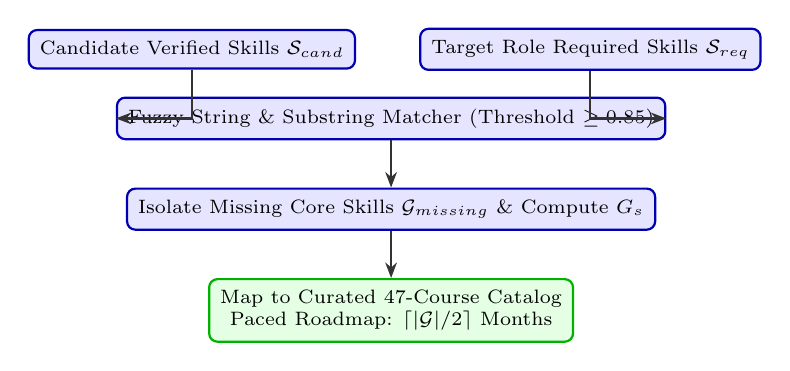
\begin{tikzpicture}[
    node distance=0.7cm,
    bnode/.style={rectangle, draw=blue!70!black, fill=blue!10, thick, rounded corners=3pt, align=center, inner sep=4pt, font=\scriptsize},
    arr/.style={-{Stealth[scale=0.85]}, thick, color=black!80}
]

\node[bnode] (c_skills) {Candidate Verified Skills $\mathcal{S}_{cand}$};
\node[bnode, right=0.8cm of c_skills] (r_skills) {Target Role Required Skills $\mathcal{S}_{req}$};
\node[bnode, below=0.6cm of $(c_skills)!0.5!(r_skills)$] (fuzzy_step) {Fuzzy String \& Substring Matcher (Threshold $\ge 0.85$)};
\node[bnode, below=0.6cm of fuzzy_step] (isolate_gap) {Isolate Missing Core Skills $\mathcal{G}_{missing}$ \& Compute $G_s$};
\node[bnode, fill=green!10, draw=green!70!black, below=0.6cm of isolate_gap] (course_map) {Map to Curated 47-Course Catalog\\Paced Roadmap: $\lceil |\mathcal{G}|/2 \rceil$ Months};

\draw[arr] (c_skills) |- (fuzzy_step);
\draw[arr] (r_skills) |- (fuzzy_step);
\draw[arr] (fuzzy_step) -- (isolate_gap);
\draw[arr] (isolate_gap) -- (course_map);

\end{tikzpicture}
\caption{Two-stage fuzzy skill matching, gap severity computation, and monthly course roadmap synthesis pipeline.}
\label{fig:gap_pipeline}
\end{figure}

\subsection{67-Feature Space Formulation}
To evaluate candidate hireability within formal hiring policies, each candidate-job pair is mapped into a 67-dimensional tabular vector:
\begin{enumerate}
    \item \textbf{Skill Coverage Features (15)}: Required skill match ratio, optional skill match ratio, gap severity $G_s$, category-level skill coverages (Frontend, Backend, Database, Cloud, DevOps).
    \item \textbf{Experience and Seniority Features (12)}: Total professional years, IT-sector tenure, role-relevant years, tenure-to-seniority ratio ($E_{rel} / Y_{req}$), career progression velocity.
    \item \textbf{Education and Credential Features (10)}: Degree tier encoding, field relevance affinity, certified credential indicators.
    \item \textbf{Assessment Telemetry Features (10)}: Component 1 screening score, Component 2 technical interview score (MCQ, descriptive, coding).
    \item \textbf{One-Hot Target Role Encodings (20)}: Binary indicators for each of the 20 canonical IT roles.
\end{enumerate}

\subsection{Gradient Boosted Decision Tree (GBDT) Formulation}
The hireability prediction model is formulated using an ensemble of $M = 300$ gradient-boosted regression trees:
\begin{equation}
F_M(\mathbf{x}) = \sum_{m=1}^{M} \eta \cdot h_m(\mathbf{x})
\end{equation}
where $\eta = 0.05$ represents the shrinkage parameter, and each tree $h_m(\mathbf{x})$ is trained on the pseudo-residuals:
\begin{equation}
r_{im} = -\left[\frac{\partial \mathcal{L}(y_i, F(\mathbf{x}_i))}{\partial F(\mathbf{x}_i)}\right]_{F=F_{m-1}}
\end{equation}
under the binary logistic cross-entropy loss function. Predicted hireability probability is recovered via the sigmoid link:
\begin{equation}
P(\text{Hireable} \mid \mathbf{x}) = \frac{1}{1 + e^{-F_M(\mathbf{x})}}
\end{equation}

\subsection{Scientific Target Definition}
\textbf{Critical Scientific Note}: In our experimental evaluation, the ground-truth binary target represents \textit{rule-based hireability eligibility} under enterprise qualification policy thresholds, because longitudinal multi-year post-hiring telemetry from real-world corporate deployments was unavailable. We explicitly avoid claiming that the model predicts whether a human recruiter will make a final job offer. Instead, the model acts as an analytical surrogate, predicting whether a candidate satisfies holistic multi-dimensional organizational qualification criteria.

\subsection{Paced Monthly Learning Pathway Synthesis}
Identified missing competencies $\mathcal{G}_{missing}$ are queried against a curated 47-course catalog covering all 20 IT domains. To avoid cognitive burnout, upskilling roadmaps enforce a strict pacing constraint of 2 skills per month:
\begin{equation}
T_{months} = \left\lceil \frac{|\mathcal{G}_{missing}|}{2} \right\rceil
\end{equation}
Prerequisite competencies (e.g., Python before Machine Learning) are sorted topologically, ensuring candidates acquire foundational proficiencies before undertaking advanced specializations.

\begin{figure}[t]
\centering
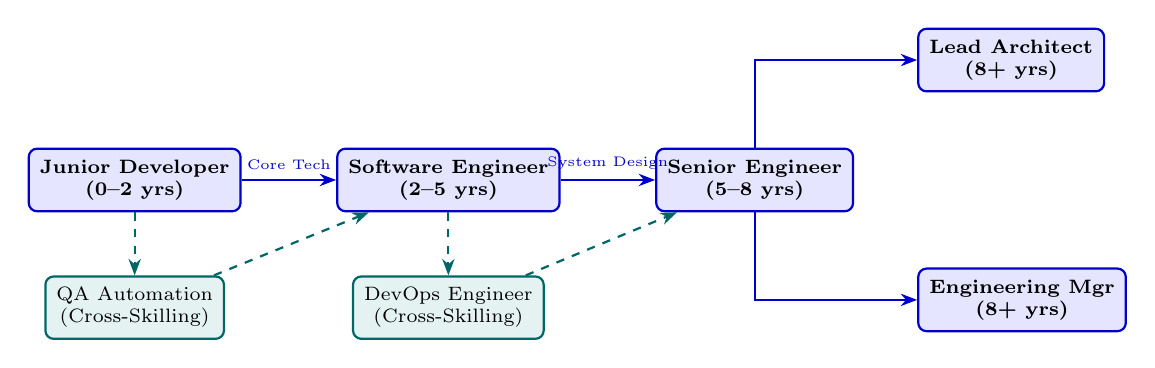
\begin{tikzpicture}[
    node distance=1.1cm and 1.3cm,
    rnode/.style={rectangle, draw=blue!80!black, fill=blue!10, thick, rounded corners=3pt, align=center, inner sep=4pt, font=\scriptsize\bfseries},
    lnode/.style={rectangle, draw=teal!80!black, fill=teal!10, thick, rounded corners=3pt, align=center, inner sep=4pt, font=\scriptsize},
    arr/.style={-{Stealth[scale=0.9]}, thick, color=blue!80!black},
    larr/.style={-{Stealth[scale=0.9]}, thick, dashed, color=teal!80!black}
]

% Nodes
\node[rnode] (junior) {Junior Developer\\(0--2 yrs)};
\node[rnode, right=1.2cm of junior] (mid) {Software Engineer\\(2--5 yrs)};
\node[rnode, right=1.2cm of mid] (senior) {Senior Engineer\\(5--8 yrs)};
\node[rnode, above right=0.7cm and 0.8cm of senior] (lead) {Lead Architect\\(8+ yrs)};
\node[rnode, below right=0.7cm and 0.8cm of senior] (mgr) {Engineering Mgr\\(8+ yrs)};

% Lateral Nodes
\node[lnode, below=0.8cm of mid] (devops) {DevOps Engineer\\(Cross-Skilling)};
\node[lnode, below=0.8cm of junior] (qa) {QA Automation\\(Cross-Skilling)};

% Transitions
\draw[arr] (junior) -- node[above, font=\tiny] {Core Tech} (mid);
\draw[arr] (mid) -- node[above, font=\tiny] {System Design} (senior);
\draw[arr] (senior) |- (lead);
\draw[arr] (senior) |- (mgr);

\draw[larr] (junior) -- (qa);
\draw[larr] (qa) -- (mid);
\draw[larr] (mid) -- (devops);
\draw[larr] (devops) -- (senior);

\end{tikzpicture}
\caption{Directed Acyclic Graph (DAG) career progression lattice modeling vertical promotional ladders and lateral cross-skilling transitions.}
\label{fig:dag_lattice}
\end{figure}

\subsection{Directed Acyclic Graph (DAG) Career Lattice}
Professional development extends beyond single-role promotions. As shown in Fig.~\ref{fig:dag_lattice}, Component 4 models occupational mobility as a directed acyclic graph $G = (V, E)$, where vertices $V$ represent job roles and directed edges $E$ encode viable transitions. Transitions are categorized as:
\begin{itemize}
    \item \textbf{Vertical Promotions}: Advancing along an established seniority ladder (e.g., Junior Developer $\to$ Software Engineer $\to$ Senior Engineer).
    \item \textbf{Lateral Cross-Skilling}: Pivoting into adjacent technological domains (e.g., Software Engineer $\to$ DevOps Engineer; QA Engineer $\to$ Software Engineer).
\end{itemize}

\section{Experimental Design and Empirical Evaluation}
\subsection{20,000-Record Candidate Dataset}
To rigorously evaluate the hireability classification engine across the full 67-dimensional feature space, we constructed a benchmark dataset of 20,000 synthetic candidate records distributed evenly across the 20 canonical IT roles (1,000 records per role). The dataset was partitioned into an 80\% training split (16,000 records) and a 20\% held-out test split (4,000 records) using stratified sampling.

\subsection{Model Benchmarking and Comparison}
We benchmarked the proposed Gradient Boosted Decision Tree (GBDT) against two competing classification architectures on identical feature splits:
\begin{enumerate}
    \item \textbf{Logistic Regression}: Linear baseline with $\ell_2$ regularization.
    \item \textbf{Random Forest}: Ensemble of 200 bagging decision trees.
    \item \textbf{Gradient Boosting (Proposed)}: 300 boosting trees, learning rate $\eta = 0.05$, max depth $= 6$.
\end{enumerate}

\begin{table}[h]
\centering
\caption{Model Architecture Comparison on 20,000 Candidate Dataset}
\label{tab:c4_model_comp}
\begin{tabular}{@{}lccccc@{}}
\toprule
\textbf{Model Architecture} & \textbf{Accuracy} & \textbf{Precision} & \textbf{Recall} & \textbf{$F_1$-Score} & \textbf{ROC-AUC} \\
\midrule
Logistic Regression & 0.8820 & 0.8410 & 0.8080 & 0.8240 & 0.9245 \\
Random Forest (200 Trees) & 0.8980 & 0.8650 & 0.8320 & 0.8480 & 0.9512 \\
\textbf{Gradient Boosting (Proposed)} & \textbf{0.9150} & \textbf{0.8840} & \textbf{0.8510} & \textbf{0.8670} & \textbf{0.9763} \\
\bottomrule
\end{tabular}
\end{table}

As documented in Table~\ref{tab:c4_model_comp}, Gradient Boosting achieves superior discriminative performance, reaching an accuracy of 91.50\%, an $F_1$-score of 0.8670, and an outstanding ROC-AUC of 0.9763, establishing high classification fidelity on tabular policy data.

\subsection{Feature Importance Breakdown}
Table~\ref{tab:c4_feature_imp} reports the top feature groupings ranked by mean Gini impurity reduction across the GBDT ensemble. Required skill match ratio and tenure-to-seniority ratio constitute the primary predictive drivers.

\begin{table}[h]
\centering
\caption{Top Predictive Feature Groups in GBDT Hireability Model}
\label{tab:c4_feature_imp}
\begin{tabular}{@{}llcc@{}}
\toprule
\textbf{Feature Group} & \textbf{Primary Variable} & \textbf{Importance} & \textbf{Impact} \\
\midrule
Skill Coverage & Required Skill Match Ratio & 0.342 & Critical Predictor \\
Experience & Tenure-to-Seniority Ratio & 0.228 & Critical Predictor \\
Assessment & Component 2 Coding Score & 0.164 & High Predictor \\
Gap Severity & Weighted Gap Index $G_s$ & 0.115 & High Predictor \\
Education & Field Relevance Affinity & 0.082 & Moderate Predictor \\
Role Encodings & 20 Role Indicator Dummy & 0.069 & Calibration Baseline \\
\bottomrule
\end{tabular}
\end{table}

\subsection{Course Recommendation Catalog and Timeline Pacing}
Table~\ref{tab:c4_courses} illustrates representative course catalog mappings and timeline projections for common missing skill profiles across three canonical roles.

\begin{table}[h]
\centering
\caption{Sample Course Mappings and Paced Learning Timelines}
\label{tab:c4_courses}
\begin{tabular}{@{}llcc@{}}
\toprule
\textbf{Target Role} & \textbf{Missing Competencies} & \textbf{Courses Mapped} & \textbf{Timeline} \\
\midrule
Software Engineer & Docker, Kubernetes & 2 Modules & 1 Month \\
Data Scientist & PyTorch, Spark, MLOps & 3 Modules & 2 Months \\
DevOps Engineer & Terraform, CI/CD, AWS, SRE & 4 Modules & 2 Months \\
Cloud Architect & TOGAF, Microservices, Security, FinOps & 5 Modules & 3 Months \\
\bottomrule
\end{tabular}
\end{table}

\section{Component Integration and Contract Interface}
Component 4 exposes REST endpoints on Port 8004. Unselected candidates from Component 3 receive a diagnostic payload:
\begin{equation}
\mathbf{y}_{c4} = \left[ G_s, \, \mathcal{G}_{missing}, \, P(\text{Hireable}), \, \text{CoursePlan}, \, \text{DAGMobility} \right]
\end{equation}
transforming an adverse hiring outcome into an immediate educational upskilling roadmap.

\section{Limitations and Threats to Validity}
\begin{enumerate}
    \item \textbf{Synthetic Policy Benchmark}: Evaluation on synthetic candidate records measures alignment with rule-based hiring policies rather than real human hiring decisions. Future work must integrate multi-year post-hire corporate retention logs.
    \item \textbf{Fixed Monthly Pacing}: Pacing at 2 skills per month assumes a standard working professional schedule; candidate life circumstances may necessitate adaptive pacing.
    \item \textbf{Static Course Catalog}: External course links and syllabi change over time, requiring automated catalog verification and periodic indexing.
\end{enumerate}

\section{Conclusion}
This paper presented Component 4 of RecruitAI: an intelligent skill gap analysis and personalized career development microservice. By integrating two-stage fuzzy skill matching, 67-feature Gradient Boosted Decision Tree hireability modeling ($\text{ROC-AUC} = 0.9763$, Accuracy = 91.50\%), a curated 47-course catalog paced at 2 skills per month, and a Directed Acyclic Graph (DAG) of career transitions, the platform bridges the divide between candidate evaluation and career mobility. By converting unselected candidate profiles into actionable learning roadmaps, RecruitAI establishes an empowering, closed-loop technical recruitment ecosystem.

\section*{Acknowledgment}
This research was conducted within the Faculty of Computing at the Sri Lanka Institute of Information Technology (SLIIT) under research project R26-IT-148.

\bibliographystyle{IEEEtran}
\bibliography{references}

\end{document}
